\documentclass[10pt,aspectratio=149]{beamer}
\usecolortheme{Calm}
\usetheme{Calm}
\usepackage{pgfplots}
\usepackage{pgfplotstable}
\usepackage[utf8]{inputenc}

\usetikzlibrary{shapes, arrows, positioning}

%------------------------------

\author{Dominique Gravel}
\title{Des changements catastrophiques à prévoir pour les écosystèmes forestiers du Québec?}
\subtitle{6ème Symposium Ouranos}
\date{\today}
\institute{UQAR - Chaire de recherche en biogéographie et écologie des métacommunautés}

%\website{http://www.chaire-eec.uqar.ca/}

%------------------------------
%------------------------------
%------------------------------
\begin{document}

	\begin{frame}[plain]
		\titlepage
	\end{frame}

%------------------------------

%------------------------------

   \begin{frame}{Enveloppes climatiques}
      \begin{columns}
         \begin{column}{0.5\textwidth}
            \begin{center}
               \includegraphics[height=0.5\textheight]{Figs/mckenney}
            \end{center}
         \end{column}
%----
         \begin{column}{0.5\textwidth}
         De nombreuses suppositions
            \begin{itemize}
               \item Distribution à l'équilibre avec le climat;
               \item Aucune démographie;
               \item Aucune interaction biotique;
               \item Aucune limite à la dispersion;
               \item Réponse linéaire et instantanée au changement climatique;               
            \end{itemize}
         \end{column}
      \end{columns}        
   \end{frame}

%------------------------------

%  \begin{frame}{Au Ministère des ressources naturelles}
%     \begin{center}
%        \includegraphics[height=0.65\textheight]{Perie2012.png}
%     \end{center}
%  \end{frame}

%------------------------------

   \begin{frame}{Objectifs}

      \textbf{Objectif général}: Cartographier et quantifier les impacts à court et long terme du changement climatique sur l'état et la productivité des forêts de l'Est du Canada. 
      \vskip 3em

      \textbf{Objectifs spécifiques}: 
      \begin{enumerate} 

         \item \textbf{Développer de nouveaux outils de modélisation pour améliorer les prédictions de l'impact des changements climatiques sur les écosystèmes forestiers};
         \item Développer de nouvelles aproches pour estimer les risques et incertitudes;
         \item Évaluer l'aptitude de différentes stratégies d'aménagement forestier à minimiser les impacts négatifs des changements climatiques. 

      \end{enumerate}
   \end{frame}

%------------------------------   
   \begin{frame}
      \begin{center}
         \includegraphics[height=0.75\textheight]{Figs/bioclim}
      \end{center}
   \end{frame}

%-------------------------------------------------------------------------------
%-------------------------------------------------------------------------------
   \section{Théorie}
%-------------------------------------------------------------------------------
%-------------------------------------------------------------------------------
   
%  \begin{frame}{Contexte théorique}
%     \begin{center}
%     \includegraphics[height=0.6\textheight]{pulliam}\\
%     \end{center}
%  \end{frame}

%-------------------------------------------------------------------------------

   \begin{frame}{Contexte théorique}{Changements de régimes catastrophiques}
      \begin{center}
      \includegraphics[height=0.6\textheight]{Figs/scheffer}\\
      \end{center}
   \end{frame}

%-------------------------------------------------------------------------------

   \begin{frame}{Contexte théorique}
      \begin{center}
      \includegraphics[height=0.6\textheight]{Figs/states}\\
      \end{center}
   \end{frame}

%-------------------------------------------------------------------------------


   \begin{frame}{Contexte théorique}
      \begin{center}
      \includegraphics[height=0.6\textheight]{Figs/early_warnings}\\
      \end{center}
   \end{frame}

%-------------------------------------------------------------------------------

   \begin{frame}
      \begin{center}
         \alert{\large{Les forêts du Québec sont-elles susceptibles à ces changements catastrophiques?}}\\
      \end{center}         
   \end{frame}

%-------------------------------------------------------------------------------

 %  \begin{frame}{Contexte théorique}
 %     \begin{center}
 %     \includegraphics[height=0.6\textheight]{svenning}\\
 %     \end{center}
 %  \end{frame}

%-------------------------------------------------------------------------------

%-------------------------------------------------------------------------------
\section{Méthodes}
%-------------------------------------------------------------------------------
%-------------------------------------------------------------------------------

   \begin{frame}{Méthodes}{Modèle}
      \begin{figure}
         \small{\input{Figs/model.tikz}}
      \end{figure}
   \end{frame}

%-------------------------------------------------------------------------------
 
   \begin{frame}{Méthodes}{Base de données}
      \begin{columns}
         \begin{column}{0.5\textwidth}
             \begin{itemize}
               \item Parcelles échantillons temporaires (MRNQ);
               \item Domtar;
               \item OMNR;
               \item Nouveau-Brunswick;
               \item FIA.
            \end{itemize}
         \end{column}
%----
         \begin{column}{0.5\textwidth}
            \begin{center}
               \includegraphics[height=0.6\textheight]{Figs/plots_map}
            \end{center}
%               \begin{itemize}
%               \item 
%               \item 5-15 ans entre les mesures
%               \end{itemize}
         \end{column}
      \end{columns}        
   \end{frame}

%-------------------------------------------------------------------------------
%-------------------------------------------------------------------------------
\section{Résultats}
%-------------------------------------------------------------------------------
%-------------------------------------------------------------------------------

%   \begin{frame}{Résultats}{Distribution des états}
%            \begin{center}
%               \includegraphics[height=0.7\textheight]{Figs/SDM_map}
%           \end{center}
%   \end{frame}

%-------------------------------------------------------------------------------

   \begin{frame}{Résultats}{Distribution des états}
            \begin{center}
               \includegraphics[height=0.7\textheight]{Figs/SDM_climate_space}
           \end{center}
   \end{frame}

%-------------------------------------------------------------------------------

   \begin{frame}{Résultats}{Effet du climat sur les transitions}
            \begin{center}
               \includegraphics[height=0.7\textheight]{Figs/Transition_climate_space}
           \end{center}
   \end{frame}

%-------------------------------------------------------------------------------

   \begin{frame}{Résultats}{Répartition actuelle}
            \begin{center}
               \includegraphics[height=0.8\textheight]{Figs/STM_map_2000}
           \end{center}
   \end{frame}

%-------------------------------------------------------------------------------

   \begin{frame}{Résultats}{Répartition en 2080}
      \begin{columns}
         \begin{column}{0.5\textwidth}
            \begin{center}
               Enveloppe climatique
               \includegraphics[height=0.6\textheight]{Figs/SDM_map_2080}
           \end{center} 
         \end{column}
%----
         \begin{column}{0.5\textwidth}
            \begin{center}
               Modèle dynamique
               \includegraphics[height=0.6\textheight]{Figs/STM_map_2080}
           \end{center} 
         \end{column}
      \end{columns}  
   \end{frame}

%-------------------------------------------------------------------------------

   \begin{frame}{Résultats}{Résilience}
      \begin{columns}
         \begin{column}{0.5\textwidth}
            \begin{center}
               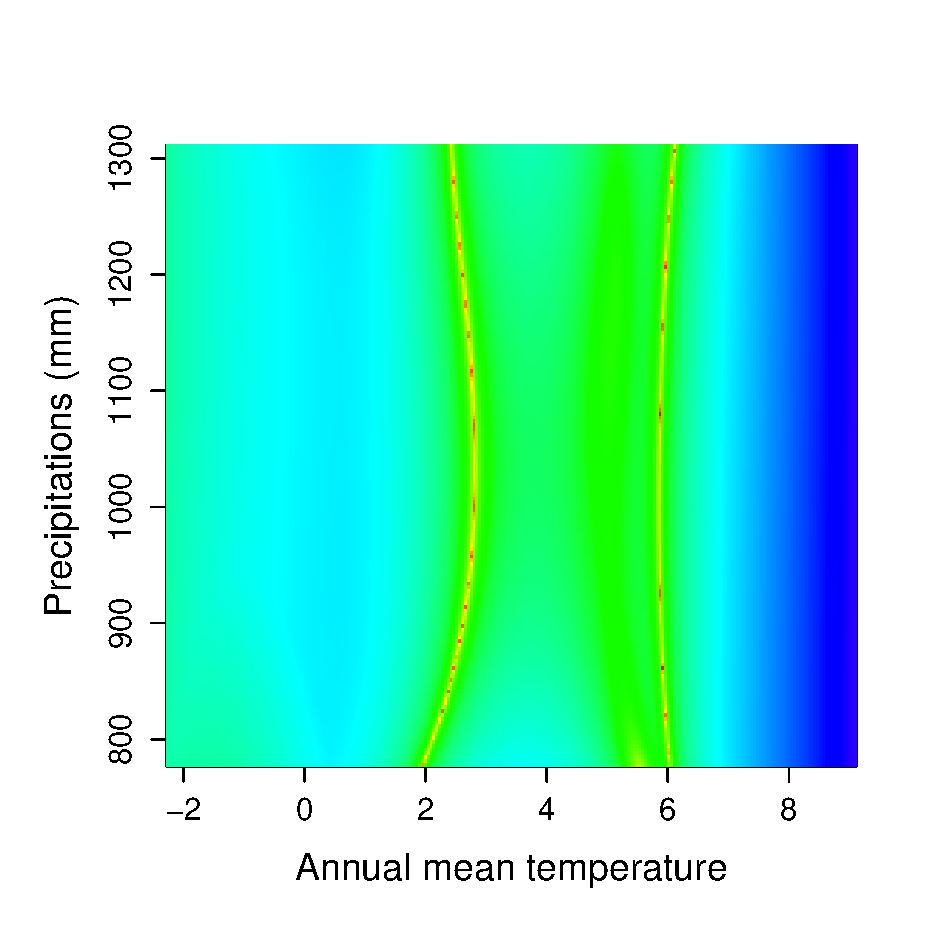
\includegraphics[height=0.6\textheight]{Figs/Eig_clim_space}
           \end{center}
         \end{column}
%----
         \begin{column}{0.5\textwidth}
            \begin{center}
               \includegraphics[height=0.7\textheight]{Figs/Eig_map}
           \end{center}
         \end{column}
      \end{columns}  
   \end{frame}

%-------------------------------------------------------------------------------

 %  \begin{frame}{Résultats}{Résilience}
 %           \begin{center}
 %              \includegraphics[height=0.7\textheight]{Figs/Eig_climate_space}
 %          \end{center}
 %  \end{frame}


%-------------------------------------------------------------------------------
%-------------------------------------------------------------------------------
\section{Discussion}
%-------------------------------------------------------------------------------
%-------------------------------------------------------------------------------

   \begin{frame}{Discussion}{Changements catastrophiques?}
      \begin{columns}
         \begin{column}{0.5\textwidth}
            \begin{center}
               \includegraphics[height=0.6\textheight]{Figs/scheffer}
            \end{center}
         \end{column}
%----
         \begin{column}{0.5\textwidth}
            \begin{itemize}
               \item Transition abrupte de la forêt tempérée à la forêt boréale;
               \item Baisse de la stabilité dans la transition;
               \item Résistance au réchauffement et augmentation des écarts;
               \item \textbf{Un maximum d'incertitude là où les changements seront les plus importants};
            \end{itemize}
         \end{column}
      \end{columns}  
   \end{frame}

%-------------------------------------------------------------------------------

   \begin{frame}{À venir}
      \begin{itemize}
         \item Analyse de la propagation des erreurs;
         \item Formulation et intégration d'un modèle démographique;
         \item Étude des vitesses de migration;
         \item Ajout de l'aménagement forestier.
      \end{itemize}
   \end{frame}

%------------------------------
   \begin{frame}{Remerciements}
       
   \textbf{Co-auteurs:} Steve Vissault, Matt Talluto, Isabelle Boulangeat;\\ 
   \vskip 1em
   \textbf{Collaborateurs:} Christian Messier, Yves Bergeron, Osvaldo Valeria, Igor Drobyshev, Frédéric Doyon, Marie-Josée Fortin, Isabelle Aubin, Daniel McKenney, Bill Parker, Steve Colombo, Charles Drever, Catherine Périé;\\ 
   \vskip 1em
   \textbf{Partenaires:} Ouranos, Parc national du Bic, CRÉ Bas-St-Laurent, Domtar, Tembec, Produits forestiers Résolu, SCF, MRN, Nature Conservancy, Corridor Appalachien;
   \vskip 1em
   \textbf{Financement:} FRQNT, CRSNG, Chaires de recherche du Canada.

   \end{frame}

%------------------------------
%------------------------------
%------------------------------
\end{document}
